\documentclass[a4paper,10pt]{article}
\usepackage[T1]{fontenc}
\usepackage[utf8]{inputenc}
\usepackage{lmodern,textcomp}
\usepackage[margin=2.2cm]{geometry}
\usepackage{amsmath,amssymb,siunitx,booktabs,graphicx,tabularx,array,enumitem,xcolor,fancyhdr}
\usepackage{tikz}
\usetikzlibrary{arrows.meta,positioning}
\usepackage[colorlinks=true,linkcolor=blue!50!black,urlcolor=blue!50!black]{hyperref}
\setlength{\parindent}{0pt}
\setlength{\parskip}{4pt}
\raggedright
\setlength{\headheight}{14pt}
\renewcommand{\arraystretch}{1.2}
\renewcommand{\tabularxcolumn}[1]{>{\raggedright\arraybackslash}p{#1}}
\setlist{nosep,leftmargin=*}
\sisetup{per-mode=symbol}
\newcommand{\file}[1]{\nolinkurl{#1}}
\newcommand{\fig}[3][0.92]{\begin{center}\includegraphics[width=#1\linewidth]{#2}\\{\small #3}\end{center}}
\pagestyle{fancy}\fancyhf{}
\fancyhead[L]{34870 Electroacoustics}
\fancyhead[R]{Lab E --- reference version (for checking)}
\fancyfoot[L]{Group 10 \quad / \quad measured 20 October 2026}
\fancyfoot[R]{\thepage}
% figures of the reference version live apart from Lab E/figures/, which is the group's own
\graphicspath{{reference_figures/}{Lab E/report/reference_figures/}}
\begin{document}
\begin{center}
{\Large\bfseries Lab E --- Loudspeaker response in free field}\\[3pt]{\large Reference version (for checking)}\\[5pt]
34870 Electroacoustics\\[4pt]
Group 10: Louis Andrianne, Sophie Kimura, Mads Rudolph\\[4pt]
Laboratory date: Tuesday 20 October 2026, 08:30--10:30 (building 354, rooms 028/025, large anechoic chamber)
\end{center}\medskip
\thispagestyle{fancy}
\fbox{\begin{minipage}{0.97\linewidth}\textbf{Reference version, not the hand-in.} This is a
complete worked version of the lab, meant for checking the group's own report and figures:
the numbers, the plots and the reasoning. Its figures sit in \file{Lab E/report/reference_figures/},
apart from \file{Lab E/figures/}, which is left for the group's own plots. Every number comes from
the measured files \file{Lab E/data/labE_<tag>.mat} and the dimensions in
\file{Lab E/matlab/labE_dims.m}, or is marked as an assumption. The group writes its own text.\end{minipage}}

\section{Purpose and theoretical basis}
The lab has two purposes: (a) to show how the frequency response and directivity of one
loudspeaker unit depend on the baffle it is mounted in, and (b) to measure the magnitude and
relative phase of the three units of the project loudspeaker (System D), which the crossover
design needs.

\subsection{Edge diffraction}
A driver in an infinite baffle radiates into half space ($2\pi$). On a finite baffle the wave
that travels along the front reaches the edge, and every edge point re-radiates a secondary
wave of opposite sign. At the microphone the direct and the edge waves add. For a driver in the
centre of a circular baffle of radius $a$ and a microphone on axis at distance $r$, all edge
points have the same path difference
\begin{equation}
\Delta = a + \sqrt{a^2 + r^2} - r \approx a \quad (r \gg a).
\end{equation}
Because the edge wave is inverted, the two waves are in phase (peak) and out of phase (dip) at
\begin{equation}
f_{\max,n} = (2n-1)\,\frac{c}{2\Delta}, \qquad f_{\min,n} = n\,\frac{c}{\Delta}, \qquad n = 1,2,\dots
\end{equation}
With the driver off-centre on a rectangle (the IEC screen), the edge distances are spread and the
secondary waves arrive at many different times, so the ripple averages out. Off axis, the edge
points of a circle are no longer equidistant from the microphone, and the ripple is smeared.
At low frequency, where the wavelength is large compared with the baffle, the sound wraps round
into full space ($4\pi$) and the on-axis level falls by up to \SI{6}{dB}: the \emph{baffle step}.
The course function \file{diffrac.m} implements Terai's method for a thin baffle with a point
source or a piston of radius $a_s$.

\subsection{Piston directivity}
A rigid piston of radius $a$ in an infinite baffle has the far-field directivity
\begin{equation}
D(\theta) = \frac{2J_1(ka\sin\theta)}{ka\sin\theta}, \qquad k = \frac{2\pi f}{c},
\end{equation}
which is \SI{-3}{dB} at $ka\sin\theta = 1.62$ and has its first null at $ka\sin\theta = 3.83$.
Dividing an off-axis response by the on-axis response on the same baffle removes the driver and,
to first order, the baffle, and leaves $D(\theta)$.

\subsection{Transfer function and phase}
The PC's line-out drives the amplifier and is fed back to line-in (channel 1, the reference);
the UMIK-1 is channel 2. The transfer function of unit $k$ in a run is
\begin{equation}
H_k(f) = \frac{\texttt{specn(:,2,k)}}{\texttt{specn(:,1,k)}} \quad [\si{Pa/V}].
\end{equation}
Its phase contains the unit's own phase, the flight time $r/c$, and a random delay
$\tau_0$ that the sound card adds to every run because playback and recording are not
synchronised. Within one run ($N_\mathrm{meas}=3$ through the switchboard) $\tau_0$ and $r$ are
common to the three units, so the relative phase $\angle(H_a/H_b)$ is valid. The course function
\file{phaseunwrap.m} adds $2\pi f d/c$ and unwraps; one distance $d$ is used for all units and
adjusted until the phases are neither all rising nor all falling.

\section{Equipment and geometry}
\begin{center}
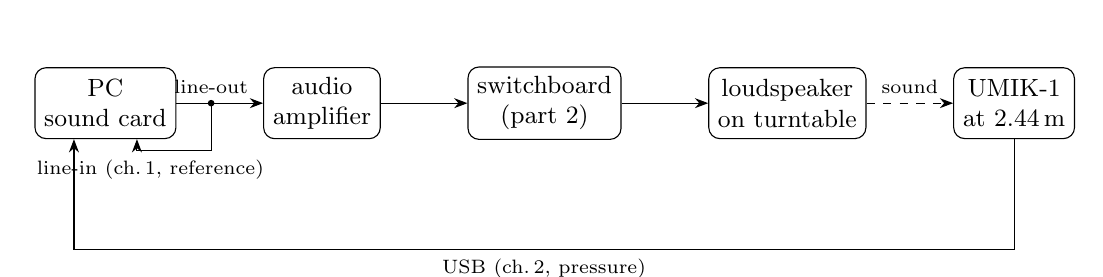
\begin{tikzpicture}[node distance=7mm and 11mm,>=Stealth,box/.style={draw,rounded corners,align=center,minimum height=9mm,font=\small}]
\node[box] (pc) {PC\\sound card};
\node[box,right=of pc] (amp) {audio\\amplifier};
\node[box,right=of amp] (sw) {switchboard\\(part 2)};
\node[box,right=of sw] (spk) {loudspeaker\\on turntable};
\node[box,right=of spk] (mic) {UMIK-1\\at \SI{2.44}{m}};
\draw[->] (pc) -- node[above,font=\scriptsize,pos=0.4]{line-out} coordinate[pos=0.4] (br) (amp);
\fill (br) circle (1.2pt);
\draw[->] (br) |- ++(-6mm,-6mm) -| node[pos=0.25,below,font=\scriptsize]{line-in (ch.\,1, reference)} ([xshift=4mm]pc.south);
\draw[->] (amp) -- (sw); \draw[->] (sw) -- (spk);
\draw[->,dashed] (spk) -- node[above,font=\scriptsize]{sound} (mic);
\draw[->] (mic.south) |- ++(0,-14mm) -| node[pos=0.25,below,font=\scriptsize]{USB (ch.\,2, pressure)} ([xshift=-4mm]pc.south);
\end{tikzpicture}
\end{center}

\begin{center}\small
\begin{tabularx}{\linewidth}{lX}
\toprule
Item & Value \\
\midrule
Microphone & UMIK-1 (miniDSP) S/N 708-0332, its own correction file, incidence 0° \\
Settings, part 1 & \SIrange{50}{20000}{Hz}, 24 lines/octave, $f_\mathrm{res}=\SI{1}{Hz}$, $N_\mathrm{av}=16$, $N_\mathrm{meas}=1$ \\
Settings, part 2 & \SIrange{50}{20000}{Hz}, 48 lines/octave, $N_\mathrm{av}=64$, $N_\mathrm{meas}=3$ (woofer, midrange, tweeter) \\
Microphone distance & \SI{2.44}{m} in both parts; height \SI{1.15}{m} above the platform in part 2 \\
Temperature & \SI{20}{\celsius}, so $c = 331.3\sqrt{1+T/273.15} = \SI{343.2}{m/s}$ \\
3\,\textquotedbl{} driver & effective diameter \SI{0.06}{m} ($a\approx\SI{3}{cm}$, rule of thumb: radius in cm $\approx$ size in inches) \\
Circular screen & radius $a = \SI{0.30}{m}$, driver centred \\
IEC screen & \qtyproduct{0.51 x 0.71}{m} (width $\times$ height), driver centre \SI{0.205}{m} from the left and \SI{0.44}{m} from the bottom edge \\
System D woofer & Scan-Speak 26W/8534G00, effective diameter \SI{0.211}{m} (data sheet), \SI{88}{L} box, vent plugged \\
System D mid/tweeter & DALI Spektor 2: 1 $\times$ 5\textonequarter\,\textquotedbl{} low/mid driver (effective diameter \SI{0.105}{m} by the rule of thumb) and 1 $\times$ \SI{25}{mm} soft dome (\SI{0.025}{m}); DALI's own crossover \SI{2600}{Hz}, \SI{84.5}{dB} (\SI{2.83}{V}/\SI{1}{m}), \SI{6}{\ohm} \\
Layout & mid/tweeter box on the woofer box at \texttt{xrel\_mid = 0.12, yrel\_mid = 0.29}; dust cover off \\
\bottomrule
\end{tabularx}
\end{center}
The DALI figures are from the manufacturer's specification page
(\url{https://www.dali-speakers.com/en-us/products/discontinued/spektor/spektor-2/}). Diameters of the
midrange and tweeter were not measured in the lab.

\section{Measurement record and quality checks}
\begin{center}\small
\begin{tabular}{lll}
\toprule
File (\file{labE_<tag>.mat}) & What & Note \\
\midrule
\texttt{box\_0}, \texttt{box\_30} & 3\,\textquotedbl{} driver in its small box & \\
\texttt{circle\_0}, \texttt{circle\_30} & circular screen & \\
\texttt{iec\_0/15/30/60} & IEC screen, off-centre & \\
\texttt{system\_0}, \texttt{system\_30} & System D, three units per file & used \\
\texttt{system\_30\_bad} & System D, 30° & rejected: up to \SI{31}{dB} off \texttt{system\_30} \\
\bottomrule
\end{tabular}
\end{center}
\begin{itemize}
\item The 60° system run was not taken.
\item Above \SI{18.4}{kHz} the UMIK channel rises by about \SI{20}{dB} in every run, including the
  bare-driver runs, while the reference channel stays flat. This is a measurement artefact, so
  all results are shown up to \SI{18}{kHz}.
\item The chamber is not anechoic at low frequency, and in part 2 the vent was plugged. Below
  about \SI{100}{Hz} the curves describe the room and the mounting rather than the drivers; the
  tweeter's response below \SI{100}{Hz} is noise.
\item The reference is the line-out \emph{before} the amplifier, so every $|H|$ includes the
  amplifier gain. The absolute levels in \si{dB} re \SI{1}{Pa/V} can therefore be compared between
  runs, but not with a manufacturer's sensitivity.
\end{itemize}

\section{Part 1: one driver, three mountings}
\subsection{Comparison of the mountings}
\fig{labE_mountings.png}{Figure 1: the 3\,\textquotedbl{} driver at \SI{2.44}{m} on the three mountings, 0° (top) and 30° (bottom). Dotted lines: the circle's first two peaks and dips from Eq.~(2).}

\begin{center}\small
\begin{tabular}{lccc}
\toprule
 & small box & circular screen & IEC screen \\
\midrule
ripple \SIrange{300}{5000}{Hz}, peak to peak, 0° & \SI{6.0}{dB} & \SI{17.3}{dB} & \SI{10.2}{dB} \\
ripple \SIrange{300}{5000}{Hz}, peak to peak, 30° & \SI{6.1}{dB} & \SI{10.5}{dB} & \SI{9.0}{dB} \\
\bottomrule
\end{tabular}
\end{center}
\begin{itemize}
\item \textbf{Small box.} From \SIrange{250}{600}{Hz} it is \SI{5.7}{dB} below the IEC screen, and from
  \SIrange{3}{8}{kHz} it is level with it ($\SI{-0.3}{dB}$). This is the baffle step: the box front is
  too small to keep the radiation in half space at low frequency. Its edges are close to the
  driver, so its own ripple is small and at higher frequency.
\item \textbf{Circular screen.} With all edge points equally far away the secondary waves add up,
  and the circle has by far the largest ripple, with deep dips (Section~\ref{sec:circle}).
\item \textbf{IEC screen.} The edges are \SIrange{0.20}{0.44}{m} from the driver, so the ripple is
  spread and smaller than on the circle, with no deep dip.
\item \textbf{At 30°} the circle's ripple falls from \SI{17.3}{dB} to \SI{10.5}{dB}, and above
  \SI{1}{kHz} the three mountings lie within a few dB of each other.
\item Common to all three: the driver's own response, a roll-off below about \SI{200}{Hz} and a peak near
  \SI{11}{kHz}.
\end{itemize}

\subsection{Circular screen: theory and diffrac.m}\label{sec:circle}
With $a=\SI{0.30}{m}$ and $r=\SI{2.44}{m}$, Eq.~(1) gives $\Delta=\SI{0.318}{m}$.
\begin{center}\small
\begin{tabular}{lcc}
\toprule
 & Eq.~(2) & measured, circle 0° \\
\midrule
first peak ($\Delta=\lambda/2$) & \SI{539}{Hz} & broad maximum \SIrange{400}{600}{Hz} \\
first dip ($\Delta=\lambda$) & \SI{1078}{Hz} & \SI{1059}{Hz}, \SI{-7.6}{dB} \\
second peak ($\Delta=3\lambda/2$) & \SI{1617}{Hz} & \SI{1679}{Hz} \\
second dip ($\Delta=2\lambda$) & \SI{2156}{Hz} & \SI{2115}{Hz} \\
\bottomrule
\end{tabular}
\end{center}
The dips are within 2\,\% of the formula. The first peak is not sharp, because the driver's own
response and the baffle step change across the same octave.

\fig{labE_circle_diffrac.png}{Figure 2: circular screen at 0° and 30° against \file{diffrac.m} for a point source and a piston with $a_s=\SI{30}{mm}$ (top two panels; the measured curve is shifted by \SI{+3.4}{} and \SI{+3.2}{dB} onto the model's mean over \SIrange{300}{5000}{Hz}). Bottom: circle minus IEC screen at 0°.}

\begin{itemize}
\item \file{diffrac.m} returns the level relative to free field, so the infinite-baffle level is
  \SI{+6}{dB}. The measured curves also contain the driver; they are shifted onto the model,
  and their shape is compared.
\item The point source keeps rippling at full amplitude to \SI{20}{kHz}. The \SI{30}{mm} piston radiates
  less along the baffle once $ka>1$ ($ka=1$ at \SI{1.8}{kHz}), so the edge waves and the ripple weaken
  at high frequency. The measurement follows the piston.
\item \textbf{The cleanest comparison} is the bottom panel: the same driver is in both the circle and the IEC
  measurement, so it cancels in the difference. Measured and modelled circle-minus-IEC agree to
  \SI{1.4}{dB} RMS (maximum \SI{3.5}{dB}) from \SIrange{300}{5000}{Hz}, including the dips at
  \SI{1029}{} and \SI{2115}{Hz}.
\item Below \SI{300}{Hz} the model and measurement part, because of the driver roll-off and the stand,
  which the thin-baffle model does not include.
\end{itemize}

\subsection{IEC screen: directivity}
\fig{labE_iec_directivity.png}{Figure 3: top, IEC screen at 0° against \file{diffrac.m} (rectangle defined relative to the driver). Bottom: 15°, 30° and 60° divided by 0° (solid) against a \SI{30}{mm} piston (dashed).}

\begin{center}\small
\begin{tabular}{lcc}
\toprule
 & piston, $a=\SI{30}{mm}$: \SI{-3}{dB} / null & measured: \SI{-3}{dB} / null \\
\midrule
30° & \SI{5.9}{kHz} / \SI{14.0}{kHz} & \SI{5.2}{kHz} / \SI{10.9}{kHz} (\SI{-17}{dB}) \\
60° & \SI{3.4}{kHz} / \SI{8.1}{kHz} & \SI{3.45}{kHz} / \SI{7.96}{kHz} (\SI{-38}{dB}) \\
\bottomrule
\end{tabular}
\end{center}
\begin{itemize}
\item At 60° the measurement lies on the rigid piston up to the null.
\item At 15° and 30° the curves follow the piston to about \SI{5}{kHz}. Above it the measured nulls come
  earlier than the piston's (the 30° null implies $a\approx\SI{38}{mm}$, and at 15° there is a dip at
  \SI{13}{kHz} where the piston has none). The cone does not move as a rigid piston there
  (break-up), which also shows as the peak near \SI{11}{kHz} in Figure~1.
\item The \SI{+3}{dB} bump near \SI{1.1}{kHz} in every ratio is the IEC screen's own on-axis dip, which
  the off-axis curves do not share: the normalisation removes the baffle only approximately.
\end{itemize}

\section{Part 2: System D}
\subsection{Magnitude}
\fig{labE_system.png}{Figure 4: System D, vent plugged. Top: the three units at 0° (solid) and 30° (dotted). Bottom: phase at 0° after \file{phaseunwrap.m} with one distance $d=\SI{-1.15}{m}$ for all units, shifted by whole turns to lie near each other at \SI{1}{kHz}.}

\begin{center}\small
\begin{tabular}{lcccc}
\toprule
mean level, \si{dB} re \SI{1}{Pa/V} & \SIrange{150}{600}{Hz} & \SIrange{1}{3}{kHz} & \SIrange{3}{8}{kHz} & \SIrange{8}{15}{kHz} \\
\midrule
woofer (Scan-Speak 26W) & 7.7 & 4.7 & 6.7 & $-9.8$ \\
midrange (Spektor 2, 5\textonequarter\,\textquotedbl) & 2.8 & 3.3 & 0.2 & $-2.2$ \\
tweeter (Spektor 2, \SI{25}{mm}) & $-19.8$ & 12.4 & 11.1 & 12.1 \\
\bottomrule
\end{tabular}
\end{center}
\begin{itemize}
\item \textbf{Woofer}: the most sensitive unit at low frequency, \SI{5}{dB} above the midrange at
  \SIrange{150}{600}{Hz}. On axis it extends to about \SI{3}{kHz}, with break-up peaks at
  \SIrange{2.5}{3}{kHz}.
\item \textbf{Midrange}: the flattest unit, within $\pm\SI{2}{dB}$ from \SI{120}{Hz} to \SI{4}{kHz}, and
  usable on axis to about \SI{12}{kHz}.
\item \textbf{Tweeter}: about \SI{9}{dB} above the midrange in its band. It is \SI{6}{dB} down from its band
  level at \SI{1.04}{kHz}, just below its resonance (the Lab D impedance has its maximum, \SI{6.7}{\ohm},
  at \SI{1.45}{kHz}).
\item \textbf{Crossings}: the tweeter crosses the woofer at \SI{958}{Hz} and the midrange at \SI{944}{Hz}.
  A crossover there would drive the tweeter at its resonance. A mid/tweeter crossover around
  \SIrange{2.5}{3}{kHz}, with about \SI{9}{dB} attenuation on the tweeter, keeps it an octave clear;
  DALI's own crossover for the Spektor 2 is at \SI{2600}{Hz}.
\end{itemize}

\subsection{Directivity}
\begin{center}\small
\begin{tabular}{lccccc}
\toprule
 & $a$ & $ka=1$ at & \multicolumn{3}{c}{30° minus 0°, measured (piston)} \\
 & & & \SIrange{1}{3}{kHz} & \SIrange{3}{8}{kHz} & \SIrange{8}{15}{kHz} \\
\midrule
woofer & \SI{105.5}{mm} & \SI{518}{Hz} & $-3.5$ ($-4.2$) & $-15.6$ ($-23.7$) & $-12.9$ ($-31.9$) \\
midrange & \SI{52.5}{mm} & \SI{1.04}{kHz} & $-1.3$ ($-0.9$) & $-7.5$ ($-10.3$) & $-16.7$ ($-24.3$) \\
tweeter & \SI{12.5}{mm} & \SI{4.37}{kHz} & $-0.9$ ($-0.1$) & $-0.7$ ($-0.4$) & $-2.5$ ($-1.9$) \\
\bottomrule
\end{tabular}
\end{center}
\begin{itemize}
\item The tweeter behaves as a \SI{25}{mm} piston.
\item Woofer and midrange beam as expected up to their first octave above $ka=1$, but less than a rigid
  piston above that: once a cone breaks up, only its inner part radiates efficiently, and its
  effective radius shrinks. The deep piston nulls are also filled by the averaging over each band.
\item For the design: the woofer is \SI{-3}{dB} at 30° near \SIrange{1.7}{1.9}{kHz} and must hand over well below
  that; the midrange holds up to about \SI{3}{kHz}, which is consistent with a crossover near
  \SI{2.6}{kHz}.
\end{itemize}

\subsection{Phase}
\begin{itemize}
\item \textbf{Compensation distance.} The single $d$ that makes the three phases smoothest
  (minimum summed phase step between adjacent lines, \SIrange{200}{15000}{Hz}) is
  $d=\SI{-1.15}{m}$; the midrange and tweeter alone give $\SI{-1.16}{m}$, the woofer
  $\SI{-1.10}{m}$.
\item $d$ is negative although the microphone was \SI{2.44}{m} away, because it absorbs the sound card's
  random delay as well as the flight time. For the same reason the other runs give unrelated
  values (\texttt{system\_30}: $\SI{-7.3}{m}$; \texttt{box\_0}: $\SI{-6.8}{m}$).
\item At $d=\SI{-1.15}{m}$ the midrange slope is slightly rising and the tweeter slope slightly falling
  between \SI{1}{} and \SI{4}{kHz}, which is the brief's stopping criterion (mixed slopes).
\end{itemize}

\fig[0.85]{labE_relative_phase.png}{Figure 5: phase of the woofer and the tweeter relative to the midrange at 0°, $\angle(H_k/H_\mathrm{mid})$, from one run. Every common delay cancels, so no compensation distance is needed.}

\begin{center}\small
\begin{tabular}{lcccccc}
\toprule
$f$ & \SI{300}{Hz} & \SI{1}{kHz} & \SI{2}{kHz} & \SI{2.5}{kHz} & \SI{3}{kHz} & \SI{4}{kHz} \\
\midrule
woofer $-$ midrange & $-12^\circ$ & $-36^\circ$ & $-58^\circ$ & $-37^\circ$ & $-54^\circ$ & $-134^\circ$ \\
tweeter $-$ midrange & $+163^\circ$ & $+162^\circ$ & $+97^\circ$ & $+85^\circ$ & $+76^\circ$ & $+90^\circ$ \\
\bottomrule
\end{tabular}
\end{center}
\begin{itemize}
\item \textbf{Woofer and midrange} are close to in phase at low frequency, and the woofer lags
  increasingly with frequency: its acoustic centre lies further back, and its low-pass roll-off adds
  phase lag.
\item \textbf{The tweeter} is nearly inverted relative to the midrange below \SI{1}{kHz}, as expected
  far below the resonance of a second-order high-pass system (\SI{+180}{\degree}), and it comes round
  to about \SI{+85}{\degree} at \SI{2.6}{kHz}.
\item The crossover filters' own phase shifts and the drivers' polarities therefore have to be chosen
  against this measured relative phase. A plain in-phase assumption would not sum correctly in the
  crossover region.
\end{itemize}

\section{Connection to Lab D}
\begin{itemize}
\item Lab D measured the electrical side of the same units: the woofer's free-air resonance
  $f_S=\SI{22.7}{Hz}$, closed-box resonance $f_C=\SI{42.0}{Hz}$ in the \SI{88}{L} box, and vent tunings
  $f_B=\SI{23.4}{}/\SI{22.8}{}/\SI{21.5}{Hz}$ for \SI{160}{}/\SI{200}{}/\SI{240}{mm} tubes. It also gave the
  complex impedances of the midrange ($R_E=\SI{4.6}{\ohm}$, resonance \SI{90}{Hz} in its box) and the
  tweeter ($R_E=\SI{3.4}{\ohm}$, resonance \SI{1.45}{kHz}).
\item Lab E gives the acoustic side: the magnitude, directivity and relative phase that the crossover
  must combine.
\item The system response is the crossover's voltage transfer (which depends on the Lab D impedances)
  times each unit's Lab E pressure per volt, summed with their phases.
\item Below about \SI{100}{Hz}, where the chamber is not anechoic and the vent was plugged, the woofer's
  response has to come from the Lab D tuning and near-field measurement.
\end{itemize}

\section{Uncertainty and conclusion}
\textbf{Main uncertainties.}
\begin{itemize}
\item \textbf{Geometry.} The mic distance is a single taped value. The 3\,\textquotedbl{} and DALI
  diameters are rule-of-thumb or data-sheet values rather than measurements. The turntable angle is
  read by eye ($\pm 2^\circ$).
\item \textbf{Room and mounting.} The chamber's lower limit and the stand and platform reflections.
\item \textbf{Measurement chain.} The UMIK correction curve and the artefact above \SI{18.4}{kHz}; noise
  where a unit is far below its band (the tweeter under \SI{300}{Hz}).
\item \textbf{Phase.} The relative phase depends on the microphone not moving within the run; it does
  not depend on $d$.
\end{itemize}

\textbf{Conclusion.} A centred driver on a circular baffle shows the regular edge-diffraction
pattern predicted by the path difference: dips at \SI{1059}{} and \SI{2115}{Hz} against
\SI{1078}{} and \SI{2156}{Hz}, and \SI{17}{dB} of ripple. The off-centre IEC screen reduces it to \SI{10}{dB},
and the small box shows the baffle step (\SI{5.7}{dB}). \file{diffrac.m} with a \SI{30}{mm} piston reproduces
the baffle difference to \SI{1.4}{dB} RMS, and the off-axis ratios follow a \SI{30}{mm} piston
(exactly at 60°) until the cone breaks up. For System D the woofer, the Spektor 2 midrange and the
tweeter were measured in one run. The tweeter is \SI{9}{dB} more sensitive than the midrange and resonates at
\SI{1.45}{kHz}, which points to a mid/tweeter crossover near \SI{2.6}{kHz} --- DALI's own choice. The
measured relative phase (tweeter $+85^\circ$ on the midrange at that frequency) is the input the crossover
design needs.

\end{document}
